\documentclass[border=3pt,tikz]{standalone}
\usepackage{amsmath}
\usetikzlibrary{3d} 
\usetikzlibrary{arrows}
\usetikzlibrary{shapes.geometric}
\usetikzlibrary{arrows,decorations.pathmorphing,backgrounds,positioning,fit,petri}
\usetikzlibrary{decorations.pathreplacing}
\usetikzlibrary{decorations.markings}
\usetikzlibrary{decorations.shapes}
\usetikzlibrary{arrows.meta}
\usetikzlibrary{quotes,angles}
\usetikzlibrary{positioning}
\usetikzlibrary{patterns} 
\usetikzlibrary{chains}
\usetikzlibrary{hobby}
\begin{document}
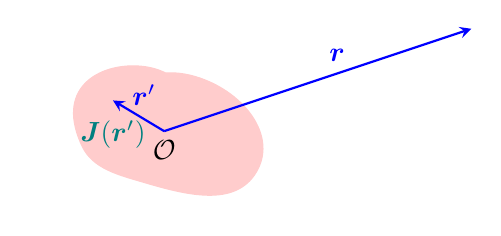
\begin{tikzpicture}[scale = 1.3, =>stealth]
    \tikzset{
        partial ellipse/.style args={#1:#2:#3}{
            insert path={+ (#1:#3) arc (#1:#2:#3)}
        }
    }

        \coordinate (N) at (1.5,3.5);
    \coordinate (O) at (0,0);
    \coordinate (P) at (-0.8, -0.15);
    \coordinate (Q) at (-0.2,-0.5);
    \coordinate (R) at (0.9,-0.4);
    % \coordinate (S) at (1.1, 0.3);
    \coordinate (T) at (0.4, 0.5);
    \coordinate (U) at (-0.3, 0.4);
    \filldraw[color=red!20, fill=red!20] (O) to [pattern=north east lines, closed, curve through = {(O) (P)  (Q)  (R)   (T) (U)}] (O);

    % \draw [->] (0,0) -- (xyz cs:x=3) node[right] {$y$};
    % \draw [->] (0,0) -- (xyz cs:y=2) node [above] {$z$};
    % \draw [->] (0,0) -- (xyz cs:z=2) node [below left] {$x$}; 
    % % \draw [very thick, teal] (0.0,2) ellipse (0.5 and 2);
      
    % \draw [-latex, very thick, teal] (xyz cs:x=0.5, y=-0.25) arc [start angle=300, end angle=660, x radius=1cm, y radius=0.3cm] node [xshift=20] {$I$};

 
    % \draw [->, thick, blue] (xyz cs:x=0, y=1) arc [start angle=90, end angle=27, x radius=1cm, y radius=1cm] node [above,yshift=15, xshift=-12] {$\theta$};    
    \draw [blue, thick, -{stealth}] (0, 0) --node[above, xshift=7, yshift=3] {$\boldsymbol{r}$} (3, 1);

    \draw [blue, thick, -{stealth}] (0, 0) --node[above, xshift=2, yshift=0] {$\boldsymbol{r}'$} (-0.5, 0.3);

    % \draw [->, red] (0, 0) -- node[above] {$a$} (xyz cs:x=-0.95, y=0, z=0);

    \node [below] at (0, 0) {$\mathcal{O}$};
    \node [below, teal] at (-0.5, 0.2) {$\boldsymbol{J}(\boldsymbol{r}')$};

\end{tikzpicture}
\end{document}